%% This is a sample manuscript marked up using the
%% AASTeX v5.x LaTeX 2e macros.

%% The first piece of markup in an AASTeX v5.x document
%% is the \documentclass command. LaTeX will ignore
%% any data that comes before this command.

%% The command below calls the preprint style
%% which will produce a one-column, single-spaced document.
%% Examples of commands for other substyles follow. Use
%% whichever is most appropriate for your purposes.
%%

%\documentclass[11pt,preprint2]{aastex}
% manuscript produces a one-column, double-spaced document:
%\documentclass[manuscript]{aastex}
%% preprint2 produces a double-column, single-spaced document:

\documentclass{emulateapj}
%\documentclass[preprint]{aastex}

\usepackage{natbib}
\usepackage{amsmath}
\bibliographystyle{apj}
\usepackage{graphicx}

%% Sometimes a paper's abstract is too long to fit on the
%% title page in preprint2 mode. When that is the case,
%% use the longabstract style option.

%% \documentclass[preprint2,longabstract]{aastex}

%% If you want to create your own macros, you can do so
%% using \newcommand. Your macros should appear before
%% the \begin{document} command.
%%
%% If you are submitting to a journal that translates manuscripts
%% into SGML, you need to follow certain guidelines when preparing
%% your macros. See the AASTeX v5.x Author Guide
%% for information.

%% You can insert a short comment on the title page using the command below.

%\slugcomment{Not to appear in Nonlearned J., 45.}

%% If you wish, you may supply running head information, although
%% this information may be modified by the editorial offices.
%% The left head contains a list of authors,
%% usually a maximum of three (otherwise use et al.).  The right
%% head is a modified title of up to roughly 44 characters.
%% Running heads will not print in the manuscript style.

\shorttitle{The HERA Dish: Beam Measurements and Science Implications}
\shortauthors{Neben et al.}

%% This is the end of the preamble.  Indicate the beginning of the
%% paper itself with \begin{document}.

\begin{document}

\title{The Hydrogen Epoch of Reionization Array Dish I: Beam Pattern Measurements and Science Implications}

%% Use \author, \affil, and the \and command to format
%% author and affiliation information.
%% Note that \email has replaced the old \authoremail command
%% from AASTeX v4.0. You can use \email to mark an email address
%% anywhere in the paper, not just in the front matter.
%% As in the title, use \\ to force line breaks.

\author{Abraham R. Neben\altaffilmark{1},
Richard F. Bradley\altaffilmark{2,3},
Aaron Parsons\altaffilmark{4},
Jacqueline N. Hewitt\altaffilmark{1},
David R. DeBoer\altaffilmark{4}
Aaron Ewall-Wice\altaffilmark{1},
Nipanjana Patra\altaffilmark{4},
Nithyanandan Thyagarajan\altaffilmark{5},
James E. Aguirre\altaffilmark{6},
Zaki S. Ali\altaffilmark{4},
Judd Bowman\altaffilmark{5},
Carina Cheng\altaffilmark{4}}

\affil{\altaffilmark{1}MIT Kavli Institute, Massachusetts Institute of Technology, Cambridge, MA, 02139 USA}
\affil{\altaffilmark{2}Dept. of Electrical and Computer Engineering, University of Virginia, Charlottesville, VA 22904}
\affil{\altaffilmark{3}National Radio Astronomy Obs., Charlottesville, VA}
\affil{\altaffilmark{4}Dept. of Astronomy, University of California, Berkeley, CA, USA}
\affil{\altaffilmark{5}Arizona State University, School of Earth and Space Exploration, Tempe, AZ 85287, USA}
\affil{\altaffilmark{6}Dept. of Physics and Astronomy, University of Pennsylvania, Philadelphia, PA}

%% Notice that each of these authors has alternate affiliations, which
%% are identified by the \altaffilmark after each name.  Specify alternate
%% affiliation information with \altaffiltext, with one command per each
%% affiliation.

%% Mark off your abstract in the ``abstract'' environment. In the manuscript
%% style, abstract will output a Received/Accepted line after the
%% title and affiliation information. No date will appear since the author
%% does not have this information. The dates will be filled in by the
%% editorial office after submission.

\begin{abstract}
The Hydrogen Epoch of Reionization Array (HERA) is a radio interferometer aiming to detect the power spectrum of 21\,cm fluctuations from neutral Hydrogen from the Epoch of Reionization. Drawing on lessons from the Murchison Widefield Array (MWA) and the Precision Array for Probing the Epoch of Reionization (PAPER), HERA is a hexagonal array of large (14\,m) dishes with suspended dipole feeds with element collecting area of 100\,m$^2$. This is the first of a series of four papers characterizing the frequency and angular response of the HERA dish element with simulations and measurements. In this work we measure the angular response at 137\,MHz using the ORBCOMM beam mapping system of \citet{neben15}. We measure collecting areas of 70--100\,m$^2$ and predict power spectrum SNRs. With optimistic foreground and analysis assumptions, HERA-127 should detect the EOR with a signal-to-noise of 25--30 with a single season of observations. Even with more pessimistic assumptions, using only previously demonstrated techniques, the significance of an EOR detection remains above $5\sigma$. Lastly we simulate foreground visibilities using numerical beam models and study the foreground distribution in Fourier space as a function of LST, and the uncertainties in these predictions due to beam modeling uncertainties.
\end{abstract}

\keywords{instrumentation: interferometers --- techniques: interferometric --- cosmology: observations --- dark ages, reionization, first stars}


\section{Introduction}
%- basics of 21cm cosmology
%    - shedding light on the unobserved Dark Ages and Epoch of
%      Reionization when the first luminous sources formed and reionized
%      the IGM
%    - MWA, PAPER, LOFAR, GMRT power spectrum experiments
%    - also global signal experiments like XX,YY,ZZ,
%        - the big challenge is recovering the signal below 4-5 orders of
%      magnitude brighter foregrounds and noise
%    - naive requirement is collecting area
%    - naive foreground removal is to subtract all low $k_\parallel$ modes

A new generation of low frequency radio telescopes is coming online with the goal of
 probing redshifted 21\,cm emission from the Cosmic Dawn. These observations will 
 complement indirect probes of the Dark Ages and Epoch of Reionization such as quasar 
 sightlines and the CMB optical depth which leave the reionization 
 history of the universe only loosely constrained. (See \citet{FurlanettoReview, miguelreview, PritchardLoebReview, aviBook, zaroubi} for reviews) Sensitivity and foreground removal are 
 the main challenges in 21\,cm observations, as the expected cosmological signal is 4--5 
 orders of magnitude fainter than Galactic and extragalactic foregrounds. Radio 
 interferometers such as the Murchison Widefield Arry (MWA) \citep{tingay13,mwascience}, the Precision Array for Probing the Epoch of Reionization (PAPER) \citep{ali2015}, the Giant Meterwave Radio Telescope (GMRT) 
 \citep{Paciga2011}, and the Low Frequency Array (LOFAR) \citep{lofar} are seeking a first detection of 
 cosmological 21\,cm emission in power spectrum measurements, where the smooth 
 frequency evolution of the foreground emission separates from the spectrally 
 unsmooth cosmological signal whose frequency dimension probes the a line of sight through the 
 inhomogenous reionizing universe.


The Hydrogen Epoch of Reionization Array (HERA) \citep[][, deBoer et al., submitted]{PoberNextGen} is drawing on lessons learned by the MWA and PAPER to reach the calibration and foreground isolation accuracy required to make a significant detection and characterization of the cosmological signal. HERA uses 14\,m diameter parabolic dishes arranged in a compact, hexagonal array to achieve coherent integration on the very low surface brightness 21\,cm signal. Redundant baselines also permit redundant calibration techniques which solve for the relative calibration between all antennas \citep{zheng14}, and use a sky model only to set the frequency dependent flux scale. In contrast, non-redundant arrays are pursuing fully sky model-based calibration schemes which risk frequency-dependent calibration systematics due to sky modeling inaccuracy \citep{braun2013}. HERA is pursuing a staged deployment of 19, 127, and finally 331 elements in progressively larger hex patterns, with scattered outriggers for imaging. A central lesson of first generation instruments is it is essential to characterize the instrument response to foreground emission lest instrument frequency dependence smear foreground power into cosmological signal modes. 

%%- but instrumental frequency structure has been recognized as critical
%  => wedge
%    - of course the bandpass and intrinsic smooth freq structure of
%      sources
%    - but also the freq-dependent sampling of the IFO
%    - sources at different zenith angles appear at different delays,
%      and thus different $k_\parallel$, increasing linearly with baseline length
%    - this gives rise to the “wedge” in cylindrically averaged power
%      spectra ($k_\perp$, $k_\parallel$)

In an ideal achromatic instrument the foreground emission would be confined to the lowest few 
line of sight Fourier modes \citep[e.g.,][]{MoralesBowmanHewittFGsub}, however  the  
interferometer's frequency-dependent point spread function smears foreground power into a ``wedge'' shaped 
region in  $(k_\perp,k_\parallel)$ Fourier space \citep{Dattapowerspec,X13, PoberWedge,MoralesPSShapes, VedanthamWedge, nithya13, CathWedge, AdrianWedge1, AdrianWedge2}. This effect is straightforward to understand for a single baseline which measures the sky intensity weighted by the complex sky fringe 
$e^{i \vec{k}\cdot\vec{b}}$, where $\vec{k}=\vec{k}(\theta,\phi,f)$ is the wave vector of 
the incident radiation, $\vec{b}$ is the baseline vector in meters, and $f$ is the observation frequency. Thus sources at different positions relative to the baseline vector manifest different 
frequency structure despite their intrinsically smooth spectra, but are geometrically limited 
by the baseline length to a maximum frequency dependence of  $e^{2\pi i f b/c}$. This limits the foreground contamination 
to a wedge shaped region in Fourier space with $k_\parallel<a k_\perp$, where $k_\perp$ and $k_\parallel$ represent spatial modes 
perpendicular and parallel to the line of sight, and $a$ is a constant depending on the observational frequency and cosmology. The complement of the wedge is knows as the ``EOR window''.

It is convenient to phrase this description in terms 
of the delay in radiation arrival at the baseline's two antennas, $\tau$, where $\tau_
\text{max}=b/c$. Sources at low delay have little frequency 
structure, while those near $\tau=\tau_\text{max}$ acquire the maximum frequency 
structure given the baseline length. 

The fact that sources acquire frequency dependence based on with their position on the sky 
tells us already that the primary beam strongly affects the aggregate frequency dependence 
of the foregrounds. The high delay regions of the sky lie near the horizon while low delay 
regions lie closer to zenith and also perpendicular to the baseline vector. \citet{nithya15} 
simulate the foreground contamination seen with a dipole beam, a phased array, and a Airy pattern,
and find that the latter suffers the least foreground leakage into
 $k_\parallel>0$ modes due to its narrow main lobe and minimal sidelobe 
levels. To be sure, all are subject to the same geometric limits on foreground frequency-
dependence limiting foreground bounding foreground emission within the wedge, but the emission from high delay is better suppressed using the 
Airy pattern leaving much of the wedge effectively empty. 

%%- the beam affects the wedge
%    - Nithya et al quantify the effects of antenna beam on the wedge
%    - wider beams like the dipole have large response at large zenith
%      angle, and thus large delays, wedge much more filled out, and
%      much more emission close to the EOR window, at risk of leaking in
%    - narrower beams like the airy have much narrower response, most
%      received emission is from low delays (near $k_\parallel=0$)
%    - but even there, emission is seen at the edge of the wedge,
%      interpreted as an effective brightening of the horizon due to the
%      very large solid angle it subtends 
%    - this structure (lots of emission from zero delay, and peak at the
%      horizon), was termed the pitchfork
%    - highlights importance of beam characterization across the entire
%      sky

From the point of view of power spectrum estimation, so long as foreground emission is perfectly contained in the wedge it is irrelevant how much or 
little of it there is, but the finite bandwidth and imperfect bandpass calibration 
of real instruments smear power beyond the geometrical edge of the wedge into the EOR 
window. Sources at higher delay appear closest to the edge of the wedge, and thus are 
most at risk of leaking into the EOR window due to these effects. In fact, 
\citet{nithya15,nithya15b} observe in simulations and then in data that while naively we might expect minimal emission 
at the very edge of the wedge because typical near-horizon beam responses are so small, 
two effects can cause a relative brightening of emission at those maximal delays, creating a characteristic ``pitchfork'' shape. This horizon 
brightening is caused by the large solid angle subtended by the near-horizon regions of the 
sky, as well as the apparent shortening of baselines when viewed nearly on axis at these elevations. 
This second effect makes intermediate length baselines of tens to hundreds of meters sensitive to the very bright diffuse 
emission would not see from near zenith. Together, these effects can overcome the decline in beam sensitivity near the horizon. 
All these considerations highlight the antenna beam as a critical design parameter for 
21\,cm observatories

%%- the design of the HERA dish
%    - small D, large N technique was enabled by moore’s law
%    - even if processing hundreds to thousands of hours of data on
%      order hundred of antennas is technically possible with parallel
%      processing and advanced data quality metrics
%    - first generation experiments are aiming for a first detection of
%      the power spectrum, even more sensitivity will be needed to
%      characterize its evolution with redshift and k, and test models
%    - HERA has thus opted for larger elements, at the expense of a
%      smaller FOV, but most of our fourier modes come from freq
%      dimension anyway
%    - a dish is preferred to a large phased array (a la SKA) as a
%      simpler antenna, with fewer degrees of freedom and reduced
%      potential for ant-to-ant variation (Neben et al)
%    - of course, elevating a feed above a dish introduces potential for
%      reflections, and thus a wigglier bandpass than that of the MWA or
%      PAPER
%    - The other papers in this series set a wiggliness spec and present
%      measurements showing it meets the spec
%    - here we focus on the angular response of the dish, ie, its beam
%      pattern

This is the first in a series of four papers detailing the HERA element. In this work we study 
angular response of the dish and its implications for power spectrum measurements. The three companion 
papers present reflectometry measurements (Patra et al., submitted) and simulations (Ewall-Wice et al., 
submitted) of the dish frequency response, as well as detailed 
foreground simulations for HERA (Thyagarajan et al., submitted). A general description to the design of the 
HERA experiment from an engineering point of view is given by DeBoer et al. (submitted). In essence, we 
require a large collecting area for
 sensitivity and minimal sidelobes and horizon response without incurring the large cost per collecting 
area of very large dishes. A dish is preferred to a large phased array as it has fewer degrees 
of freedom and reduced potential of antenna-to-antenna variation (Neben et al 2015b, 
submitted). These factors naturally lead to a 14\,m diameter parabolic dish with a dipole 
feed suspended at prime focus. The 352 dishes are positioned in a compact, hexagonal 
array permitting redundant baseline calibration and coherent integration in $
\vec{k}$ space \citep{omniscope,ali2015}. 
%The smaller field of view of the HERA dish relative to that of the PAPER dipole or the MWA tile does not limit sensitivity in Fourier space as most leverage on high $k$ modes is from line of sight modes anyway \citep{PoberNextGen}.

%%- roadmap
%    - we use orbcomm to measure the dish beam pattern and calculate
%      collecting area, verify the focus
%    - then we assess the science implications in delay space, comparing
%      different models and power spectrum approaches
%%- how sensitive are we to accurate beam models?
%    - what must we show about the HERA dish to confirm that it will
%      allow us to reach the science we want?
%    - large collecting area is a given
%    - minimal sidelobes and horizon response
%    - how accurately must we verify the beam model? different analyses
%      require different levels of beam modeling fidelity
%    - HERA’s hexagonal grid permits redundant baseline calibration
%      which is agnostic to the antenna beam, as long as all are the
%      same. ant-to-ant variation adds noise to the redundant
%      calibration, likely much smaller than that incurred in MWA sky
%      model calibration 
%    - the PAPER delay spectrum technique and 1D clean is even agnostic
%      to ant-to-ant variation, as it cleans out all sky emission within
%      the horizon limits on a per baseline basis
%    - an imaging analysis (a la MWA) relies on foreground subtraction,
%      and containment of residuals in the wedge, and the subtraction
%      step is much more sensitive both to accurate modeling of the mean
%      beam and to ant-to-ant variation (Neben et al)
%    - the general questions we address in this paper
%        - the questions are: does the main lobe shape agree with the
%          model (need good model for imaging and FG subtraction)
%        - are the sidelobe levels and horizon response sufficiently
%          small to mitigate pitchfork effect and foreground leakage?

In this paper we first characterize the angular response of a prototype HERA dish at the National Radio 
Astronomy Observatory--Green Bank. We use the beam mapping system of \citet{neben15} to 
measure the 137\,MHz beam pattern using the ORBCOMM satellite constellation. We obtain beam 
measurements out to zenith angles of $\sim60^\circ$ where the beam response is -35\,dB relative to zenith, and compare with different numerical models. We characterize the dish beam at various feed heights to map out the focus and study beam errors due to feed misalignment. We compute the collecting areas and implied EOR power spectrum sensitivities of our measured beams. After verifying our numerical models, we consider the science implications of these 
beam patterns by foreground delay spectra at different baseline lengths and observing conditions to study when the horizon brightening effect is strongest, and thus, when foreground are must at risk of leaking into the EOR window.

In detail, we discuss the electromagnetic design and modeling of the dish in Section 2. We present the 
experimental setup of the beam mapping experiments and discuss their systematics, then 
review the ORBCOMM beam measurement system, in Section 3. We present our power pattern 
measurements in Section 4, and study the science implications of these beam measurements for foreground power spectra in Section 5, then conclude with discussion in Section 6.

\section{Dish Design and Modeling}

\subsection{Design of the HERA Dish}

We review here the design of the HERA dish, and refer to DeBoer et al. (submitted) for details. 
The 14\,m HERA dish design is a departure from the large N--small D approach used by 21\,cm 
observatories like PAPER and the MWA. Both observatories are actively pursuing power 
spectrum analyses using several year data runs, but the sheer data volume makes 
characterization and removal of systematics, as well as repeated or complimentary analyses, 
challenging. A larger element was chosen for HERA primarily to reduce correlation and data processing costs. 

The HERA element is a 14\,m diameter parabolic dish ($f/D\approx0.32$) with a dual-polarized dipole feed (Fig. \ref{fig:feedphoto}) suspended at prime focus. The dish surface is formed by sheets of wire attached to PVC tubes attached to supports at the edge of the dish and to a hub at the base. The feed is suspended with cables attached to three telephone poles around the dish. For feed maintenance purposes, a door is engineered into the dish surface on one mesh panel. The dipole stands 17\,in below a 78\,in diameter circular mesh back plane surrounded by a 30\,in deep cylinder. The cylinder is offset 0.5\,in from the back plane. The feed is designed to make the beams for both polarizations more similar to each other, and also to taper the dipole beam towards the edge of the dish to mitigate dish-dish coupling.  The nominal dish focus is at 4.5\,m from the dish surface, though numerical dish models including the feed predict the focus is closer to 5.3\,m. 

Feed/dish optimization studies are ongoing and these parameters may change in the final HERA array, but in this work we use the feed with these dimensions and study the beam with the feed suspended at different heights. We study the position of the dish focus, the shape of the main lobe, the magnitude of the dish sidelobes, the degree of beam symmetry, the actual dish/feed efficiency (i.e., collecting area), and the expected level of antenna-to-antenna variation.

\begin{figure}[h]
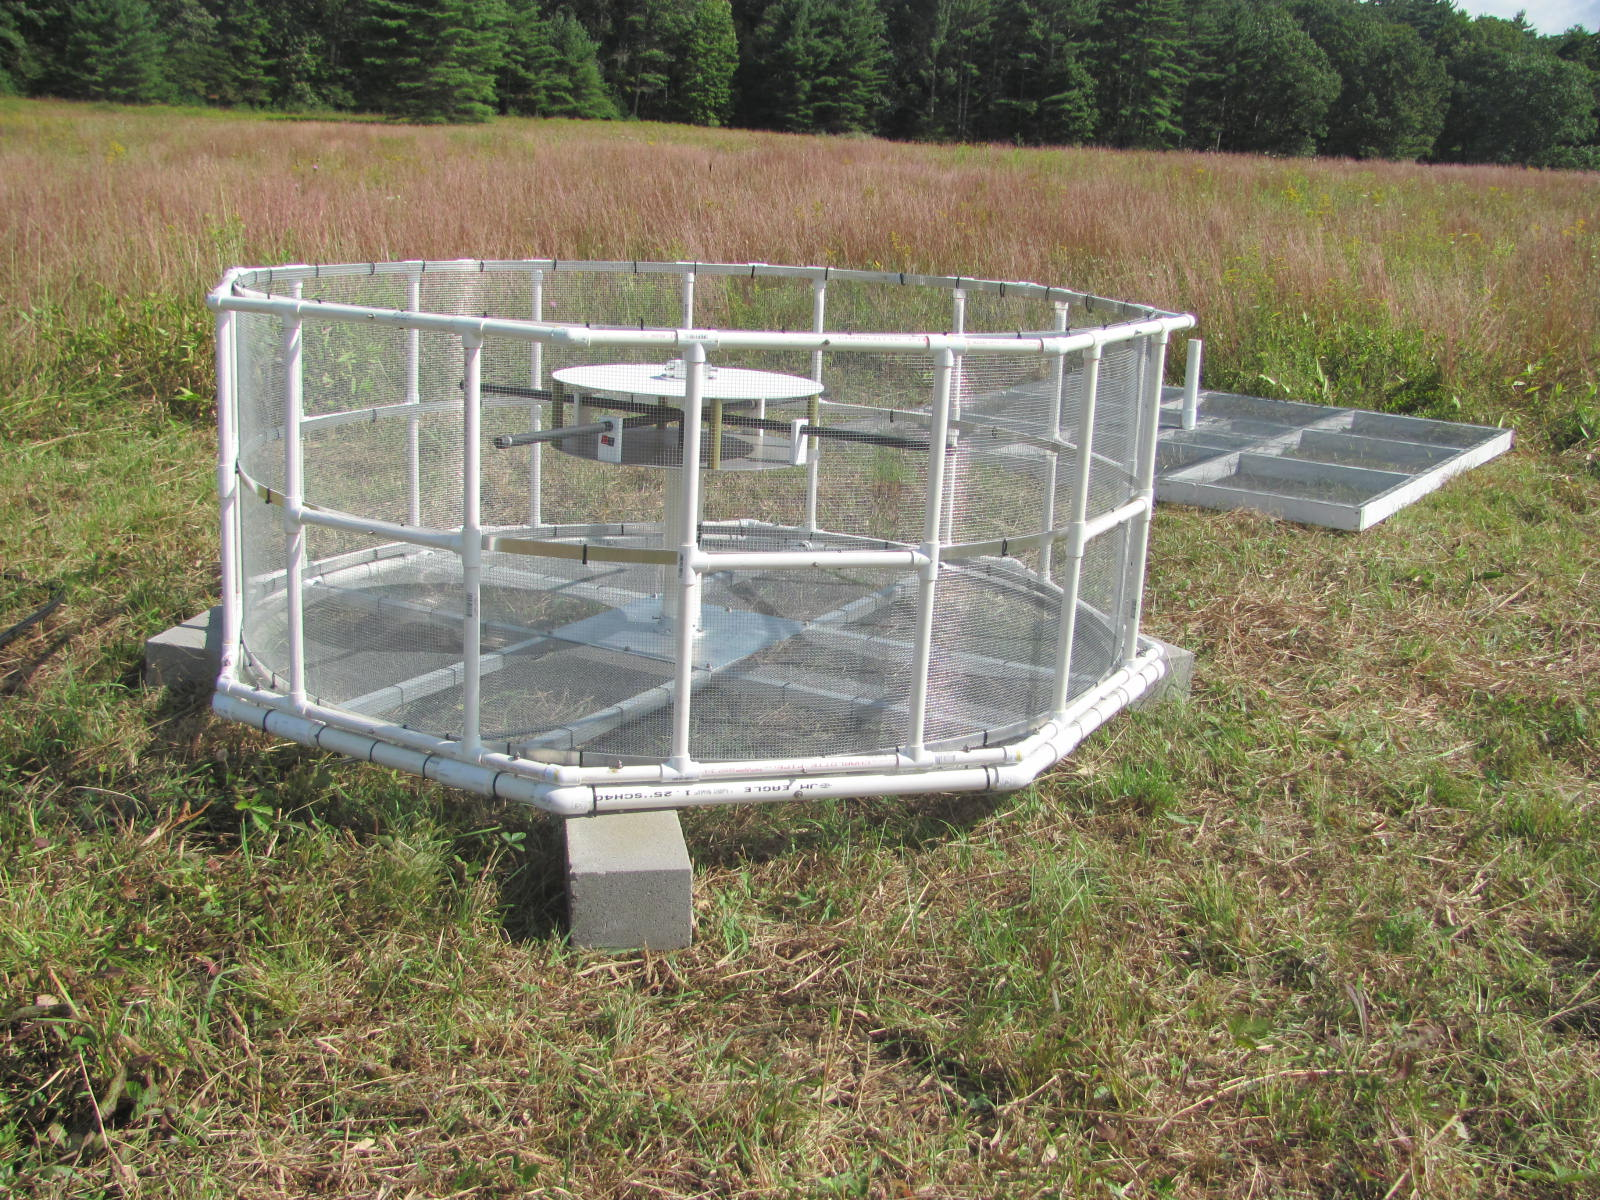
\includegraphics[width=3.4in]{feed.jpg}
\caption{Prototype HERA feed set up outside the dish for preliminary characterization. This feed revision consists of a dual-polarized sleeved dipole offset 17\,in from a 78\,in diameter back plane, surrounded by a 30\,in deep cylindrical skirt.}
\label{fig:feedphoto}
\end{figure}

One cost of using fewer large antenna elements is a smaller field of view, but this is a 
small effect for 21\,cm power spectrum analyses as our leverage on $k$ modes comes primarily from $k_\parallel$ modes along the line of sight (in the frequency dimension). More significant is frequency structure introduced by time domain reflections between the suspended feed detailed by Ewall-Wice et al. (submitted) with simulations and Patra et al. (submitted) with zenith reflectometry measurements.

\subsection{Dish Modeling}
\label{sec:dishmodels}

\begin{figure*}
\centering
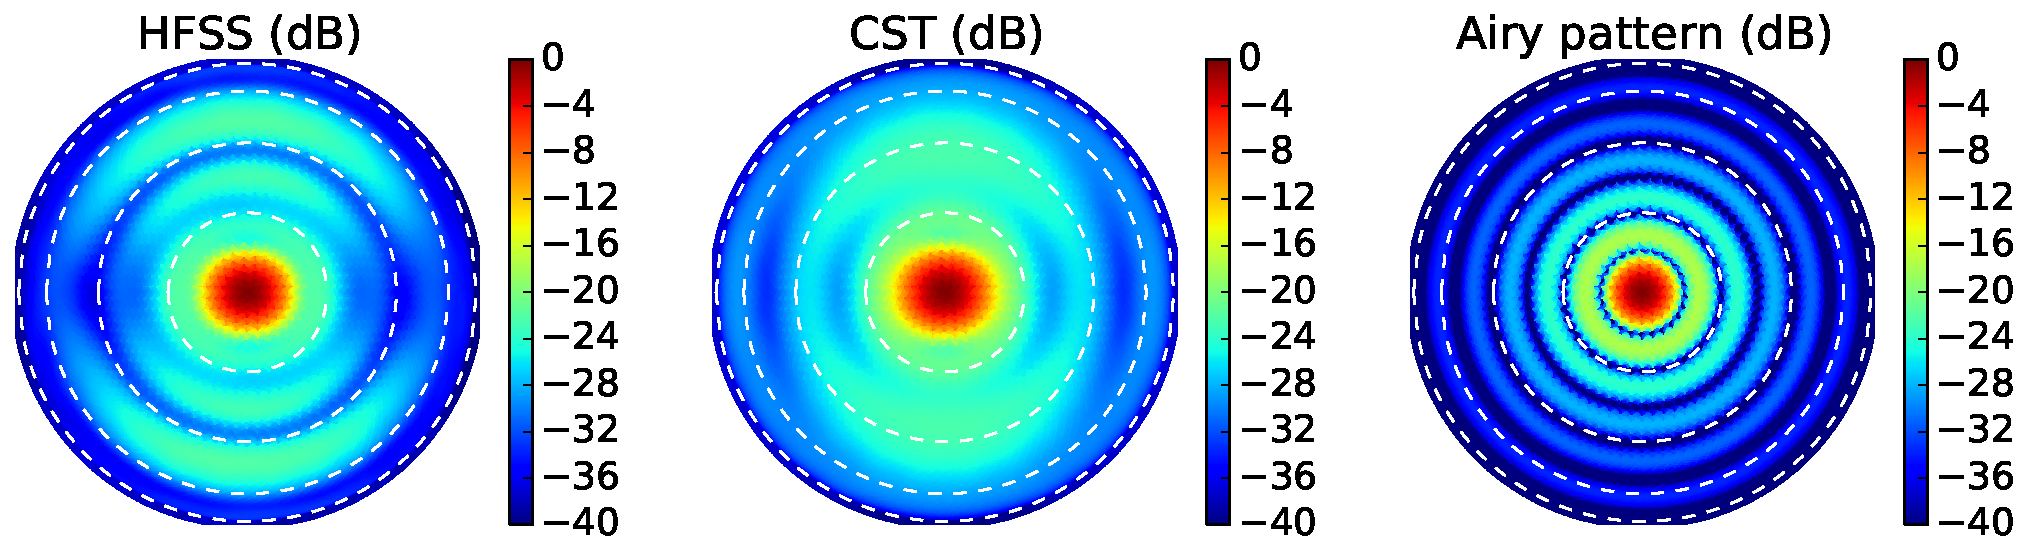
\includegraphics[width=7in]{dave197_rich195_airy_beams.pdf}
\caption{Simulated dish power patterns at 137\,MHz (Sec. \ref{sec:dishmodels}) using HFSS (left) and CST (middle) are shown beside an ideal Airy pattern for a 14\,m diameter dish for comparison.}
\label{fig:modelbeams}
\end{figure*}

We numerically model the HERA dish in both HFSS and in CST, making slightly different assumptions, in order to study the dependence of the beam pattern on modeling imperfections. In particular, we suspect that the near horizon beam response, which sets the level of horizon brightening, is quite sensitive to modeling assumptions. Modeling is also useful to probe the best focus of the dish--feed system. The nominal focus is at 4.5\,m given that the dish has $f/D=0.32$, though the feed back plane and skirt are expected to move the focus slightly.

The HFSS model uses a 14\,m paraboloid with $f/D=0.32$ as the dish, with a 1\,m hole at vertex. In reality the 1\,m diameter at the vertex is filled with concrete and supports the PVC pipes which suspend the mesh panels, but we effectively assume here it is perfectly absorbant.  The feed is modeled as a PAPER dipole suspended 17\,in below a 78\,in diameter circular backplane inside a 30\,in deep skirt hanging 0.5\,in below the backplane. All these surfaces are modeled as solid aluminum, as are the dipole ``sleeves'', circular disks just above and below the dipole plane designed to broaden its frequency response. The dipoles themselves is modeled as a copper pipe of diameter XX, we neglect the dielectric PVC in which the copper pipe is actually enclosed. In the simulations, we excite one of the dipoles using a modal port and measure the total gain response in each direction to 137.5\,MHz radiation.

In the CST model we again model the dish as a 14\,m diameter solid aluminum paraboloid with $f/D=0.32$ but now neglect the 1\,m hole at zenith, effectively assuming the concrete and earth ground behind it are perfectly reflective. The actual material properties are somewhere in between, though difficult to predict theoretically. The feed model has the same dimensions as in the HFSS model. The simulations are done by exciting one of the dipoles with band-limited noise (100--200\,MHz). The beam pattern is then obtained at a given frequency using a farfield monitor after the excitation pulse energy within the structure decays to below -80\,dB.

\section{Experimental Setup}

\subsection{ORBCOMM Beam Mapping System Review}

We briefly review the beam mapping system detailed by \citet{neben15}, then discuss 
application of system for HERA dish measurements. The system 
takes advantage of the 137\,MHz communications satellites operated by ORBCOMM Inc. 
as bright point sources which, by virtue of their number ($\sim30$), short orbital periods 
($\sim90$ minutes), and orbital precession cover $\sim$65\% of the visible sky in just a few 
days. The coverage from the Green Bank site is limited by the fact that the satellites' orbital inclinations are all less 
than $45^\circ$. 

Unlike celestial source beam measurements, where the flux may be 
assumed constant over the timescale of the measurement, satellite fluxes can vary rapidly 
due to changing distance, orientation, and transmission power. To correct for this, we 
measure the satellite flux in each ground polarization (EW and NS) using a simple, well-
modeled reference antenna. Comparison of this measured power with that observed in the 
Antenna-Under-Test (AUT) gives the AUT beam response in the direction of the satellite. 
An equivalent interpretation of the measurement is that the power ratio between the AUT and the reference 
antenna gives the relative beam response in the satellite direction, and multiplication by 
the reference antenna model yields the desired AUT response. As discussed in 
\citet{neben15}, this procedure correctly measures the response of the AUT to unpolarized radiation
 despite the fact that satellite signals are generally polarized.

In detail, we measure the dual-polarization RMS power received by each antenna in 512 2\,kHz 
channels across the 137--138\,MHz band. Each band power is averaged over $\sim0.2$
\,sec. There are 0--3 satellites above the horizon at any given time transmitting on different 
$\sim15$\,kHz wide sub-bands in 137--138\,MHz. By observing at many different 
frequencies, we probe the beam response in all these directions simultaneously. We 
compute the satellite positions using the orbital elements published by Celestrak
\footnote{http://www.celestrak.com/NORAD/elements/orbcomm.txt} and the orbital 
integrator \texttt{predict}\footnote{http://www.qsl.net/kd2bd/predict.html}. However, the 
satellite frequencies vary occasionally to avoid interference within the constellation. 
\citet{zheng14} use interferometric phases to identify and exclude times when multiple 
satellites are in view. As our data acquisition system makes only total power 
measurements, we instead use an ORBCOMM interface box (typically supplied to 
commercial users of the network) to sync with passing satellites and record their identifier 
and transmission frequency during each pass.

In this way, beam measurements are built up along satellite tracks over the course of 
several days of integration, yielding typically 200--300 satellite pass. Each pass is 
processed separately to identify and exclude times of low signal-to-background when the 
satellite is low in the sky or in the off state of of a pulsing sequence. At those times, then 
satellite flux no longer dominates over that of the diffuse Galactic background, and a 
power measurement no longer probes the response in only the satellite direction. The beam 
measurements are then gridded in horizontal coordinates in HEALPix \citep{healpix} with a resolution of 
$1.8^\circ$ (nside=32). As a last quality control step to reject errant beam measurements 
due to RFI, for instance, we keep only the central 90\% of $\sim50$ measured beam 
values in each HEALPix cell.


\subsection{HERA--Green Bank: A three-element prototype array}

A 3-element HERA engineering prototype is being constructed at the National Radio 
Astronomy Observatory--Green Bank. We performed the beam measurements presented in 
this work on the first of these dishes to be constructed, future work will characterize its beam in the presence of the other two dishes once they are constructed. The prototype array is situated in Galford Meadow, approximately 1\,km southwest of the Green Bank Telescope. Note that unlike the full HERA site in the Karoo Desert Radio Astronomy Reserve in 
South Africa, the Green Bank site has trees and foothills, as well as moist ground. Our beam measurements
are sensitive to these effects in addition to the construction imperfections of real world dishes.

\begin{figure}[h]
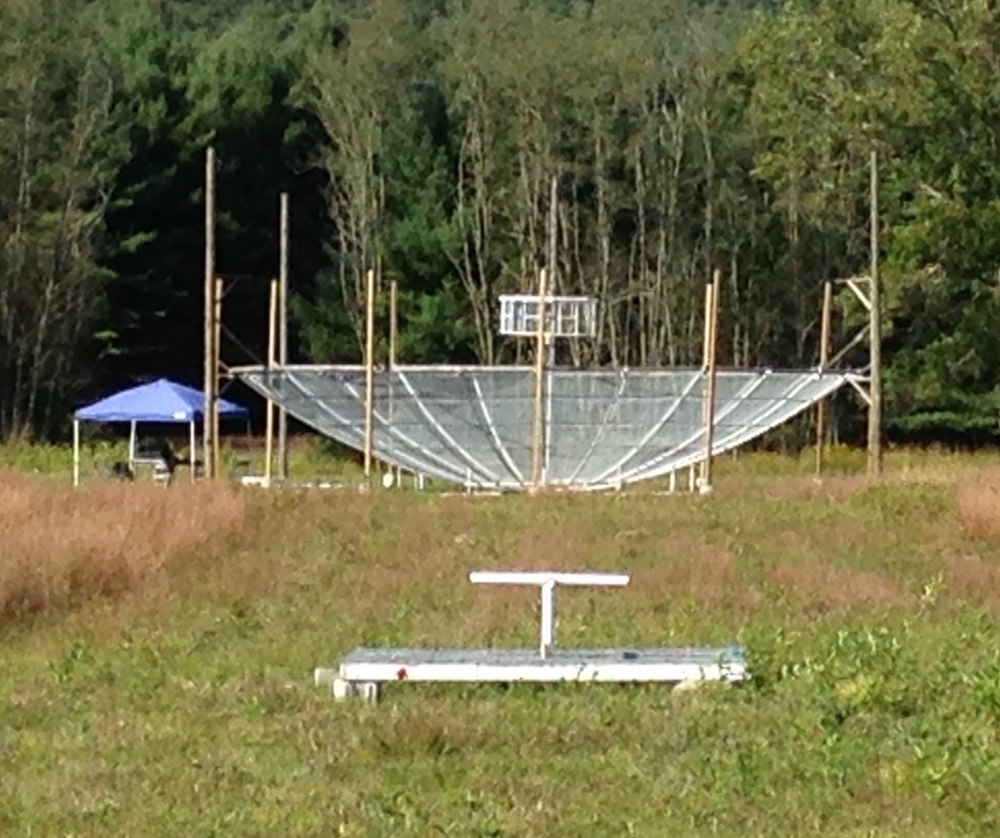
\includegraphics[width=3.4in]{ref_dipole_and_hera_dish.jpg}
\caption{The dish with its suspended feed is seen in the back, 50\,m north of one of the reference antennas used in the null experiment to study systematics. The experiment is conducted in Galford Meadow at NRAO--Green Bank.}
\label{fig:greenbankdishphoto}
\end{figure}

We use a simple dual-polarization dipole as our reference antenna. The dipole is constructed out of copper tubing covered by PVC for protection, mounted above a 2\,m $\times$ 2\,m ground plane. See \citet{neben15} for details. During the dish measurements the dipole is positioned 100\,m due south of the dish, though we experiment with other locations at first in our to characterize the environmental systematics of these measurements, as detailed in the next section. Figure \ref{fig:greenbankdishphoto} shows the dish with suspended feed 50\,m north of one of the reference antennas.

\subsection{Assessing Experimental Systematics}

\begin{figure*}[h]
\centering
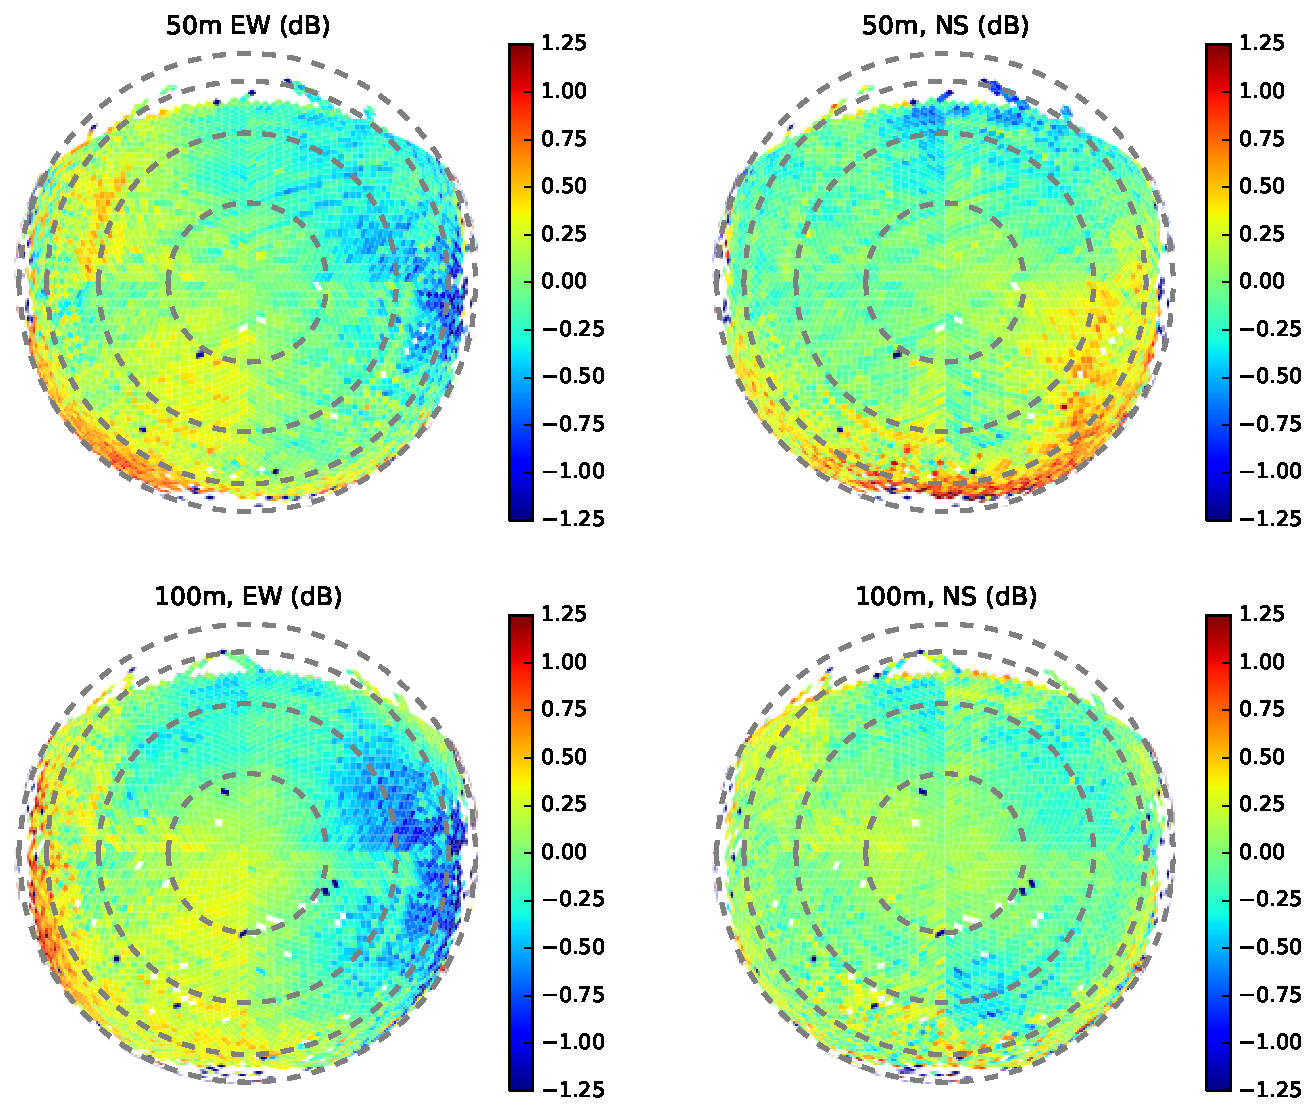
\includegraphics[width=6.5in]{null_expt_rel_beam_maps.pdf}
\caption{We characterize the accuracy of the beam measurement system through null experiments in which a second reference antenna is taken as the AUT and ratio of both reference antenna power patterns is measured for EW (left) and NS (right) polarizations. The reference antennas are separated by 50\,m from each other and from the HERA dish in the first experiment (top), and by 100\,m from each other and from the HERA dish in the second experiment (bottom).}
\label{fig:nullexptplots}
\end{figure*}

As in \citet{neben15}, we assess systematics using a ``null experiment'' in which we use a second reference dipole as the antenna-under-test (AUT). Taking the ratio of its measured power pattern with the model beam pattern amounts to a ratio of the raw power responses received by the two antennas as a function of satellite direction. This probes the level of environmental systematics (i.e., reflections and varying ground properties) and antenna fabrication imperfections which affect each antenna differently. This is not a probe of modeling imperfections common to both antennas, but we expect such errors to be subdominant as the physical properties of the antenna are easier to characterize, and thus simulate, than misalignments and local environmental effects. 

As we are not able to replace the HERA dish with a reference antenna, we run two null experiments with both reference dipoles deployed (1) 50\,m apart on a NS line, 50\,m south of the HERA dish; and (2) 100\,m apart on a NS line, 100,m south of the HERA dish. Figure \ref{fig:null1} shows the  results from these experiments in the form of the ratio of the power responses of the two antennas. We collected roughly 100 satellite passes. Systematics at the few percent level are observed in  within $20^\circ$ of zenith, and at the $10--20\%$ level farther out. The magnitude and angular distribution of these systematics changes modestly as the separation is changed, suggesting that the reference dipoles differ largely due to intrinsic differences, with some environmental variation. In any case, these fractional errors propagate directly into our measured dish power patterns.

\section{Dish Measurements}

\subsection{Power pattern measurements}

\begin{figure*}[t]
\centering
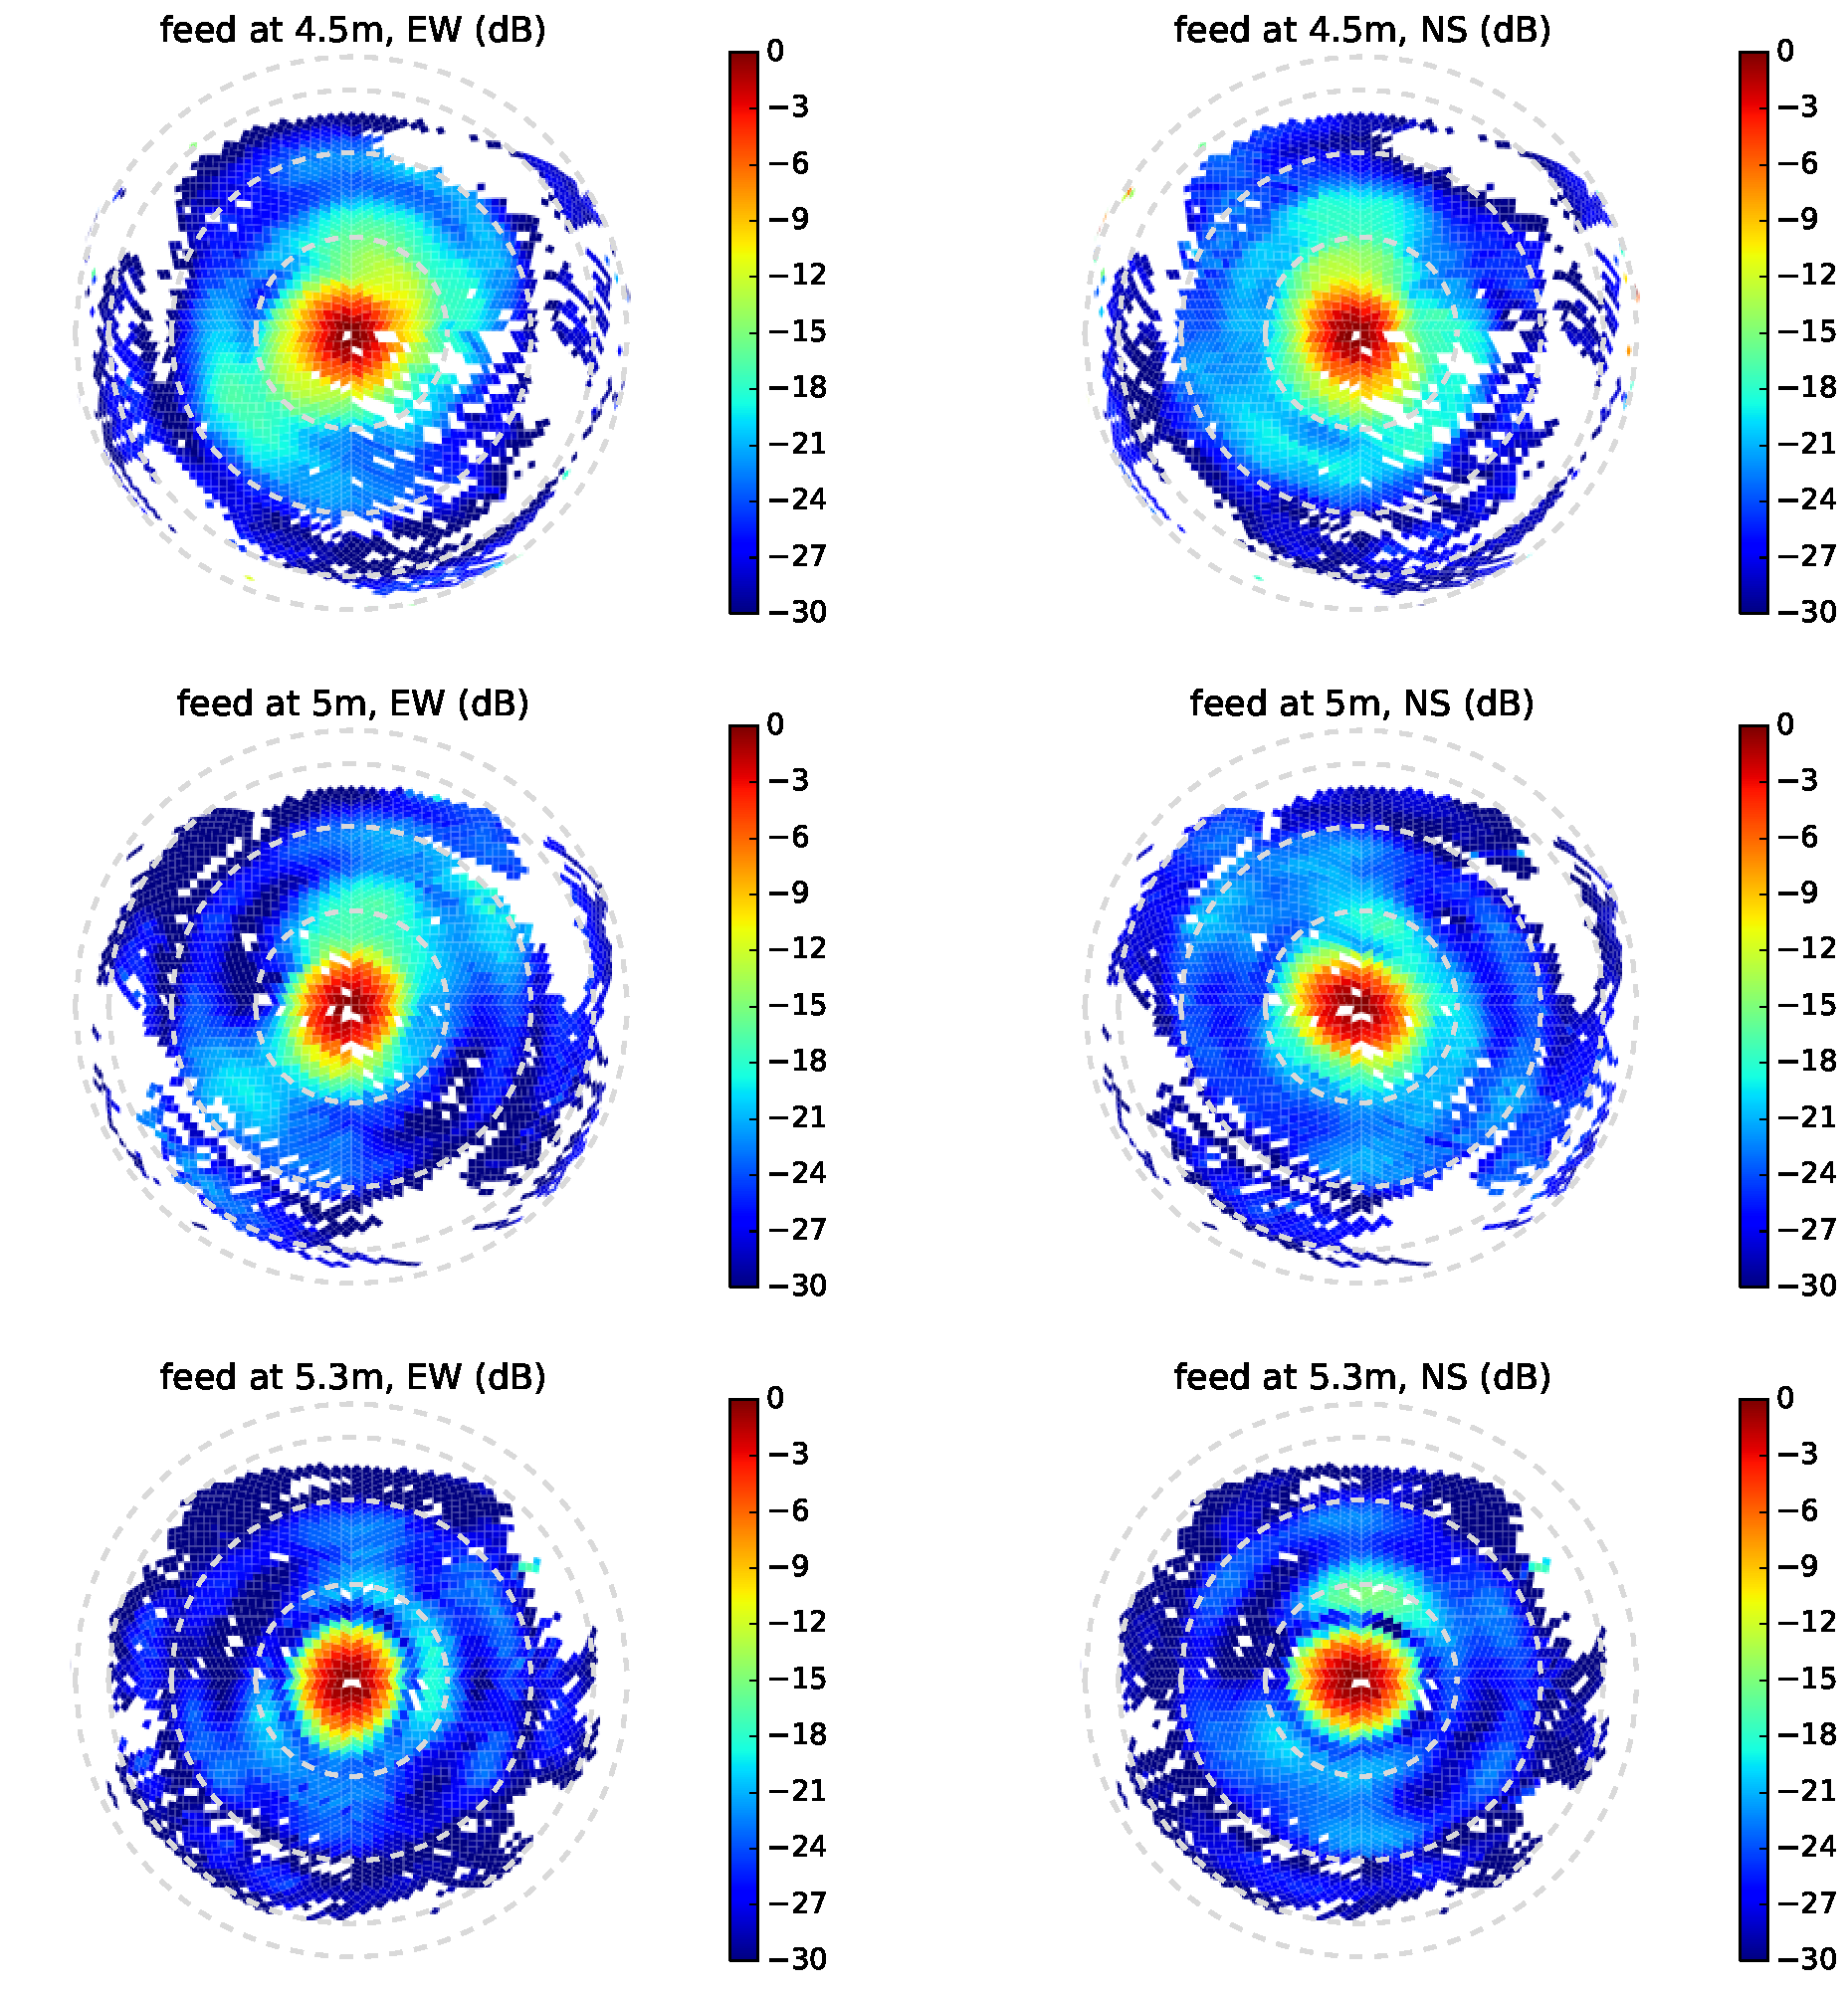
\includegraphics[width=6.5in]{measured_beams_and_models_maps.pdf}
\caption{Measured dish power patterns at various feed heights for the EW (left panel) and NS (right panel) instrumental polarizations. The sidelobes shrink and the main lobe narrows as the feed is raised, confirming that the focus of the dish/feed system is higher than the 4.5\,m ideal focus of the parabolic dish.}
\label{fig:measuredbeammaps}
\end{figure*}

\begin{figure*}[t]
\centering
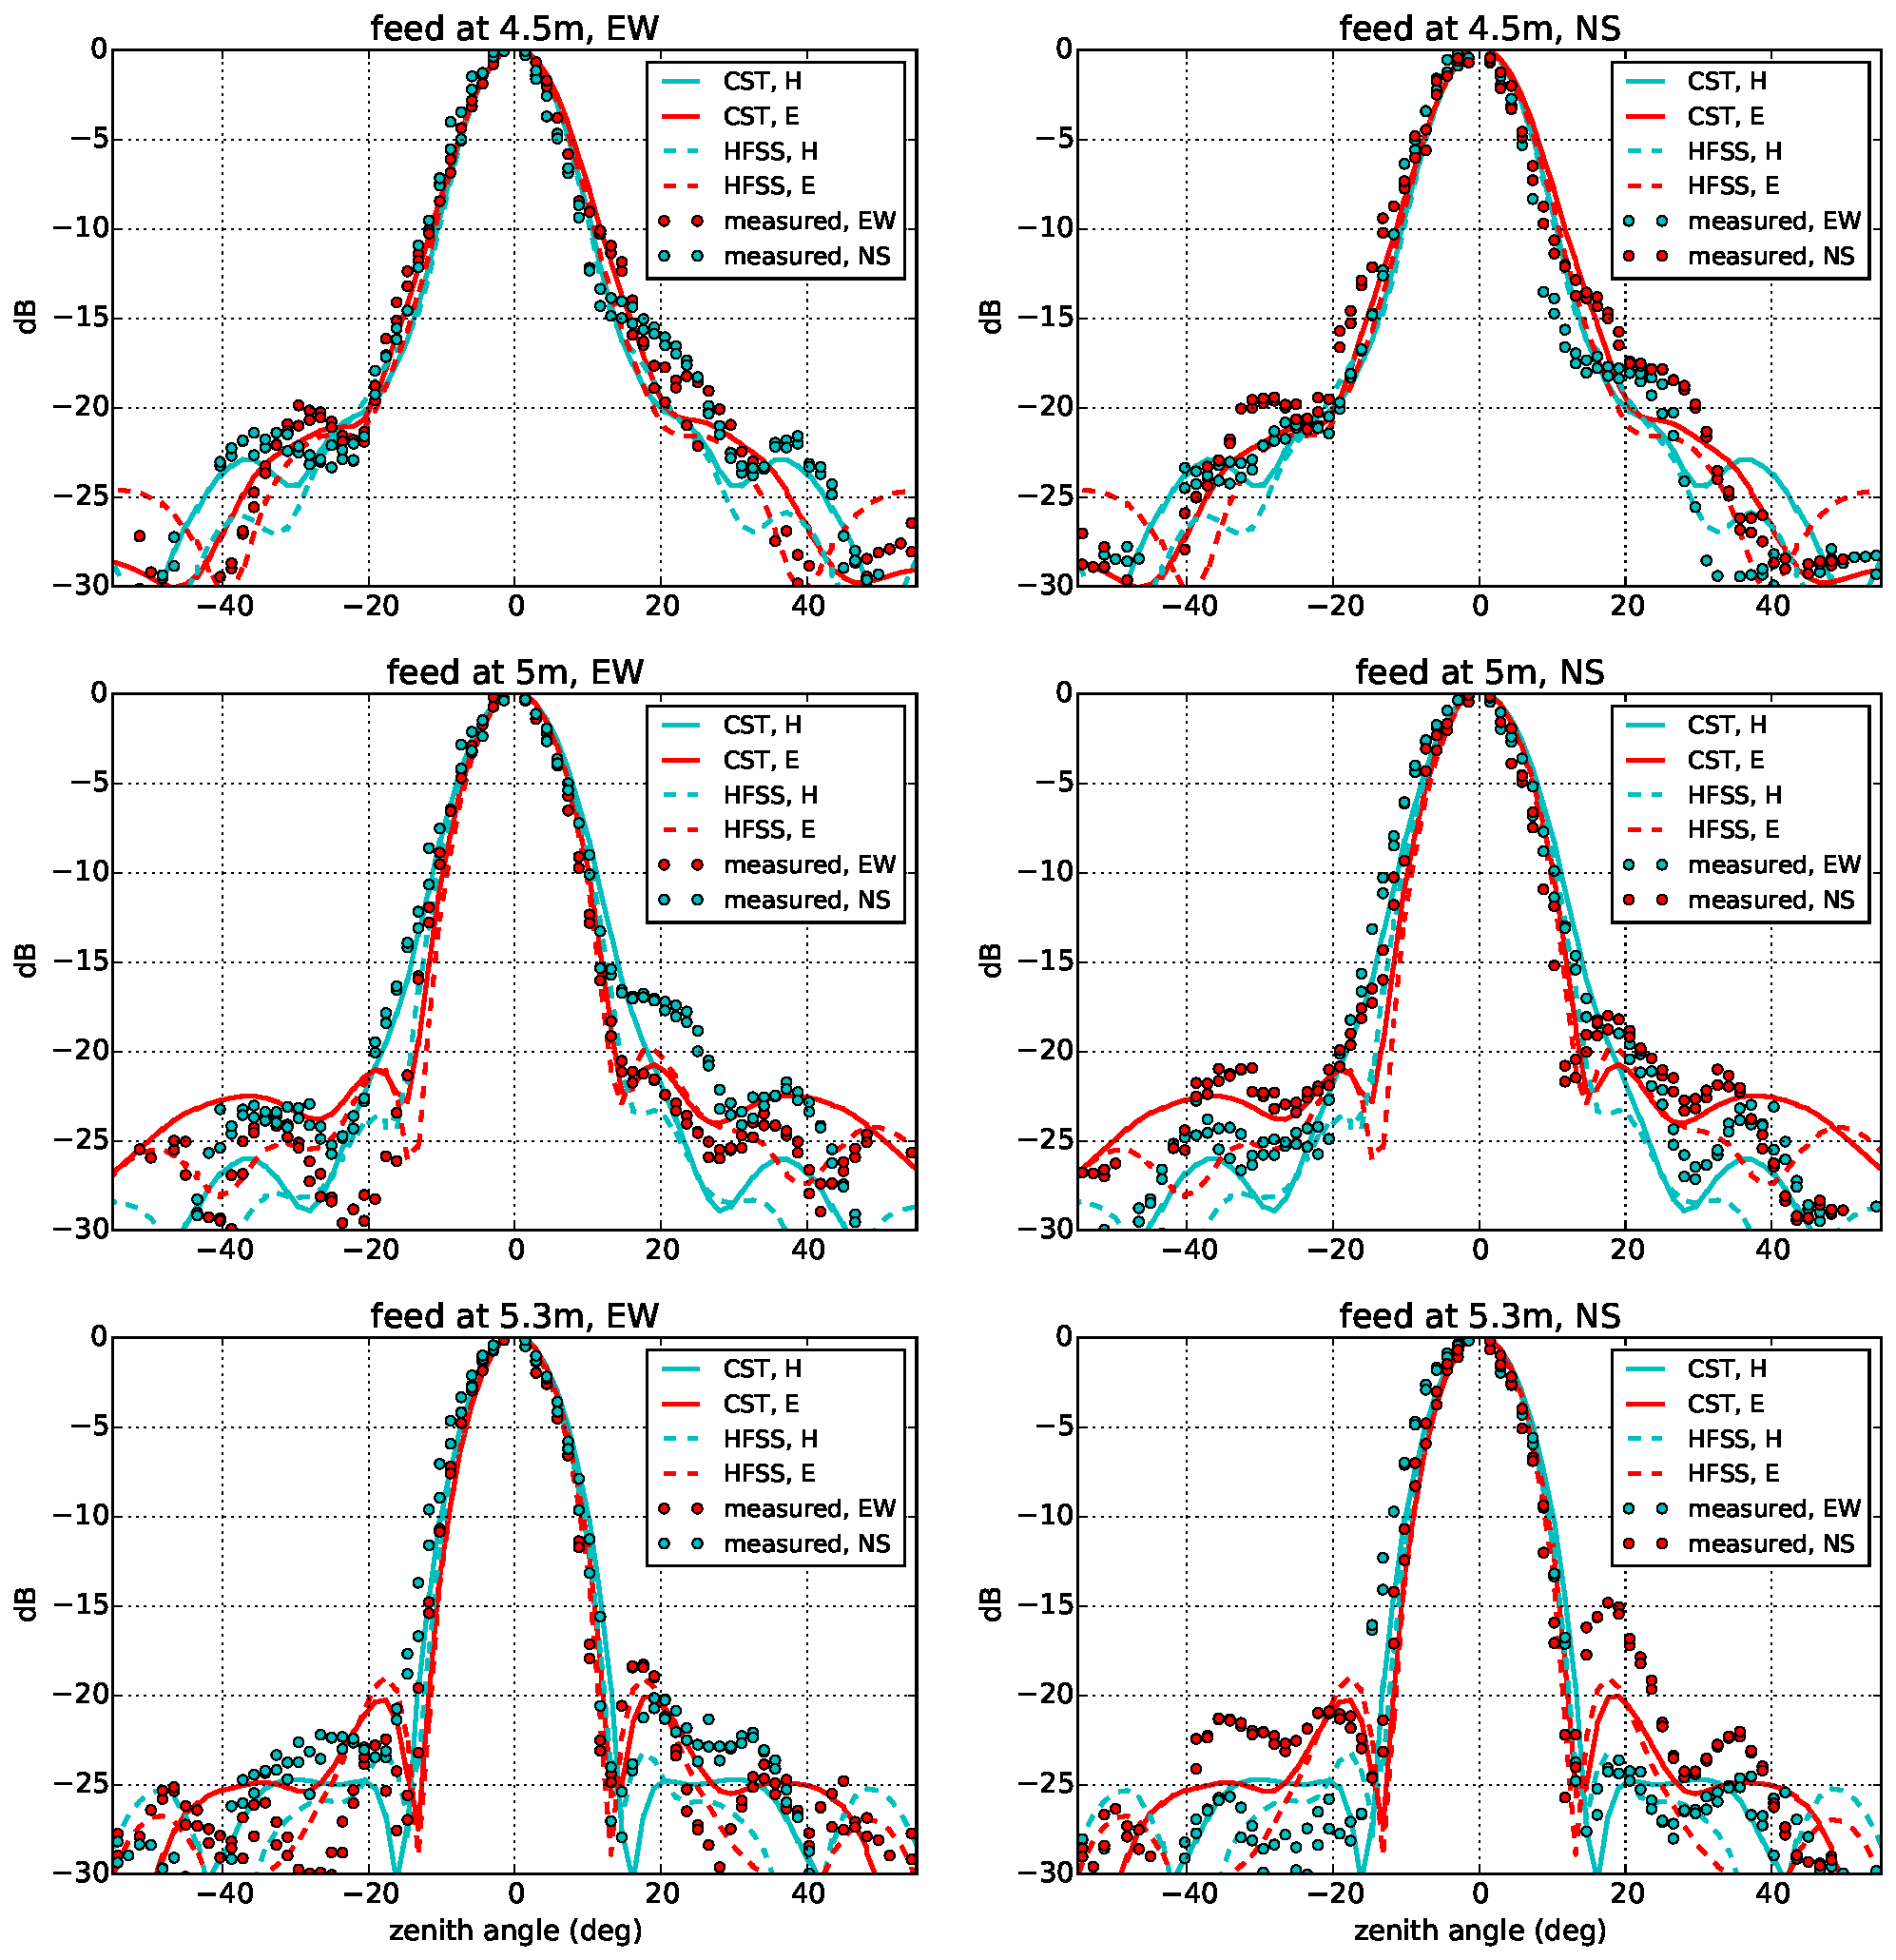
\includegraphics[width=6.5in]{measured_beams_and_models_slices.pdf}
\caption{Slices through the E and H planes through the measured dish power patterns (points) and numerical models (curves). The measured beams agree with both models in the main lobe out to zenith angles of 15--20$^\circ$, but begin to deviate in the sidelobes at the 0.1--0.5\% level of the beam.}
\label{fig:measuredbeamslices}
\end{figure*}

We make three dish power pattern measurements with the feed at different heights: (1) 4.5\,m, the nominal dish focus; (2) 5.0\,m, an intermediate focus; and (3) 5.3\,m, the numerically determined focus of the dish/feed system, where all heights are measured from the dish surface to the feed back plane. In each configuration we collect data for 2--4 days, obtaining roughly 200 satellite passes. We exclude times when the received power is within 20\,dB of the background level determined at between passes, and then grid measured beam values into 1.8$^\circ$ HEALPix cells on the sky, rejecting outliers in the top or bottom 5\% in each cell as a final guard against rare satellite identification problems or ADC saturation issues.

Figure \ref{fig:measuredbeammaps} shows the measured power patterns for these three feed heights for the EW (left panel) and the NS (right panel) feed polarization. These maps are plotted in sine-projection with dashed circles marking zenith angles of $20^\circ$, $40^\circ$, $60^\circ$, $80^\circ$. The sky coverage in these dish measurements extends out to typically $\theta\sim50-60^\circ$. Beyond that the ORBCOMM flux is sufficiently attenuated relative to diffuse galactic emission that a power ratio measurement between the two antennas is no longer a clean probe of their gains in the direction of the satellite. At these zenith angles, the beam sidelobes are roughly -30\,dB, and are trending downward at the edge of the measured region.

The roughly $10^\circ$ main lobe narrows slightly as the feed is raised from 4.5\,m to 5.3\,m, and the sidelobes shrink both in size and in amplitude, confirming the numerically predicted focus of 5.3\,m. As expected, the EW main lobes are slightly wider in the NS direction. In theory, the only asymmetric part of the dish is the dipole feed, so the overall beam should have a $180^\circ$ azimuthal symmetry. We observe deviations from this symmetry at the few dB level in the sidelobes, suggesting dish surface and/or feed imperfections given that the systematics identified in the null experiment are smaller. 

Figure \ref{fig:measuredbeamslices} shows slices through the E and H planes of these power patterns along with the HFSS and CST numerical models discussed earlier. As in the previous plot, the EW and NS beams are shown it the left and right panels, while the different feed heights are shown in the different rows. The data agree with both models to within a dB in the main lobe, but begin to diverge in the sidelobes at zenith angles of $20^\circ$ and larger. Here the evolution of the sidelobes as the feed is raised is again seen starkly, as is the fact that the main lobes are slightly wider along the H planes than along the E planes. 

\subsection{Sensitivity}

We compute the effective collecting areas of these beam patterns by first interpolating over unmeasured cells and smoothly extrapolating the power pattern to the horizon. These operations produce a realistically smooth beam which reaches roughly -30\,dB at the horizon, as suggested by the numerical models. The collecting area is related to the power pattern as
\begin{equation}
	A=\frac{\lambda^2 B(0,0)}{\int B(\theta,\phi)d\Omega}
\end{equation}

The collecting areas range are shown in Table 1 along with the maximal collecting area achieved by the Airy pattern for a 14\,m dish. The measured collecting areas are a 30--50\% lower than the geometric area. This is in line with expectations given that the Airy pattern has the largest possible collecting area, equal to the dish cross section, and the feed's backplane and cylindrical skirt reduce it. However we opt for this reduction over added collecting area in order to reduces the azimuthal beam asymmetry and minimize the cross-coupling between adjacent dishes.

 \begin{table}[h]
 \caption{ \label{table:collectingareatable}Collecting area (m$^2$) of measured 137\,MHz beams and corresponding power spectrum SNR for HERA-127.}
\begin{tabular}{| l | l | l |}
\hline
Beam & $A_\text{eff}$ (m$^2$) & SNR (pess, mod, opt)\\
\hline
  Airy pattern & 155 & 9.1, 11.0, 37.2  \\
  %CST sim & 67.0 &  \\
  %Measured, feed at 4\,m & 44.3 &  \\
    Measured, feed at 5.3\,m & 97.9 & 8.2, 8.3, 29.2 \\
    Measured, feed at 5\,m & 82.6 & 6.8, 6.9, 26.5 \\
    Measured, feed at 4.5\,m & 73.6 & 6.4, 6.5, 24.8 \\ 
  \hline
\end{tabular}
\end{table}

We run 21cmSense\footnote{https://github.com/jpober/21cmSense} to compute the overall SNR of a power spectrum detection with one season (6 hours per night for 180 nights) of HERA-127 data. To input these collecting areas into 21cmSense, we convert these measured dish collecting areas into effective dish diameters, which we input as the \texttt{dish\_size\_in\_lambda} parameter. We predict the SNRs with optimistic, moderate, and pessimistic foreground assumptions. In the optimistic case, $k$ modes inside the same $uv$ pixel are added coherently, and all modes whose frequency dependence is larger than that of source at the edge of the main lobe are used. In the moderate case, $k$ modes inside the same $uv$ pixel are added coherently and only modes whose frequency dependence falls outside of the horizon plus a buffer are used. In the pessimistic case, all baselines are added incoherently and only modes outside the horizon plus a buffer are used.

The SNRs computed with the measured collecting areas fall from 9--11 for the Airy pattern  to 6--8 in the pessimistic and moderate cases. In the optimistic case, the SNR falls from 37 with the Airy pattern to 24--29 with the measured collecting areas. In all cases this reduction is a loss of sensitivity, but a power spectrum detection is still always very significant at the 6$\sigma$ level or better.

\section{Foreground Delay Spectrum Simulations}
\label{sec:foregrounds}

We turn in this section to the effects of the beam power pattern on the apparent frequency dependence of the foregrounds. Thyagarajan et al., (submitted) discuss the apparent frequency dependence of foregrounds in more detail as well as methods to mitigate it such as delay space CLEANing. We focus in this section on the uncertainties in these foreground power spectrum simulations due to beam modeling uncertainties, but we must first discuss these foreground simulations themselves and their dependence on observing conditions. 

We simulate foreground power spectra using different primary beam models at various local sidereal times (LSTs). We use frequency-independent model beams (evaluated at 137\,MHz) to isolate the interferometric foreground frequency dependence. The added frequency dependence of the changing overall gain and beam shape versus frequency is addressed by the other papers in this series. Given that our measured dish power patterns agree well with both numerical models (HFSS and CST) in the main lobe but deviate in the sidelobes, and that these models make somewhat different assumptions about the dish surface, we take them as a representative pair of possible dish models. We use a feed height of 5\,m, a compromise between collecting area and risk of coupling to adjacent dishes. We also include the Airy pattern for comparison as in \citet{nithya15}. Beam models with weaker response near the horizon (such as the Airy pattern) downweight sources in this direction of high apparent frequency dependence. This reduces the magnitude of emission near the edge of the EOR window, reducing the risk it leaks inside. We use the per-baseline approach of \citet{parsons12a,parsons12b}, simulating visibilities measured by specific baselines as a function of frequency, then computing the Fourier transform over frequency (delay transform) and normalizing the result into a cosmological power spectrum following \citet{nithya15}. 

In detail, we simulate visibilities for each beam model at various LSTs, modeling the sky as the sum of the Global Sky Model \citep{gsm} and the Culgoora \citep{Slee1995} and MWA Commissioning Survey \citep{MWACS} point source catalogs. We use a frequency spacing of 1\,MHz, sufficient to characterize delays within and just outside of the horizon limits on both baseline lengths we are concerned with, 14\,m and 42\,m. We use a total bandwidth of 100\,MHz (50\,MHz after applying the Blackman-Harris window) centered on 150\,MHz. This bandwidth is larger than the 10\,MHz thought to be safe from signal evolution over redshift, but is the bandwidth used in the wide band delay space foreground CLEAN of \citet{paper32,paper64}.

Figure \ref{fig:delayspec} (top panel) shows simulated foreground delay spectra at various LSTs using the nominal HFSS beam. As all these LSTs are high galactic latitudes far from the galactic center, the total visibility power (the level of the zero delay mode) varies only by a factor of a few over these LSTs on both baseline lengths (14\,m (left panel), 42\,m (right panel)). However the negative delay horizon limit (corresponding to the western horizon) has a peak that varies by over three orders of magnitude on the 14\,m baseline and by two orders of magnitude on the 42\,m baseline, demonstrating the stark difference in horizon brightening when the galaxy is just above versus just below the horizon. 

In this figure we perform the approximate conversion from delay $\tau$ to $k_\parallel$, which we plot as a second $x$-axis at the top of the plot. For these short baselines, $k_\parallel$ may be converted to $k$ by adding $k_\perp=0.005$ for the 14.6\,m baseline or $k_\perp=0.02$ for the 42\,m baseline in quadrature. These numbers are small compared to the range of $k_\parallel$ plotted, and thus we interpret the $k_\parallel$ axis as simply the $k$ axis, and plot a 1D model power spectrum computed using 21cmFast \citep{21cmfast} as a dotted line for comparison. 

\begin{figure*}[h]
\centering
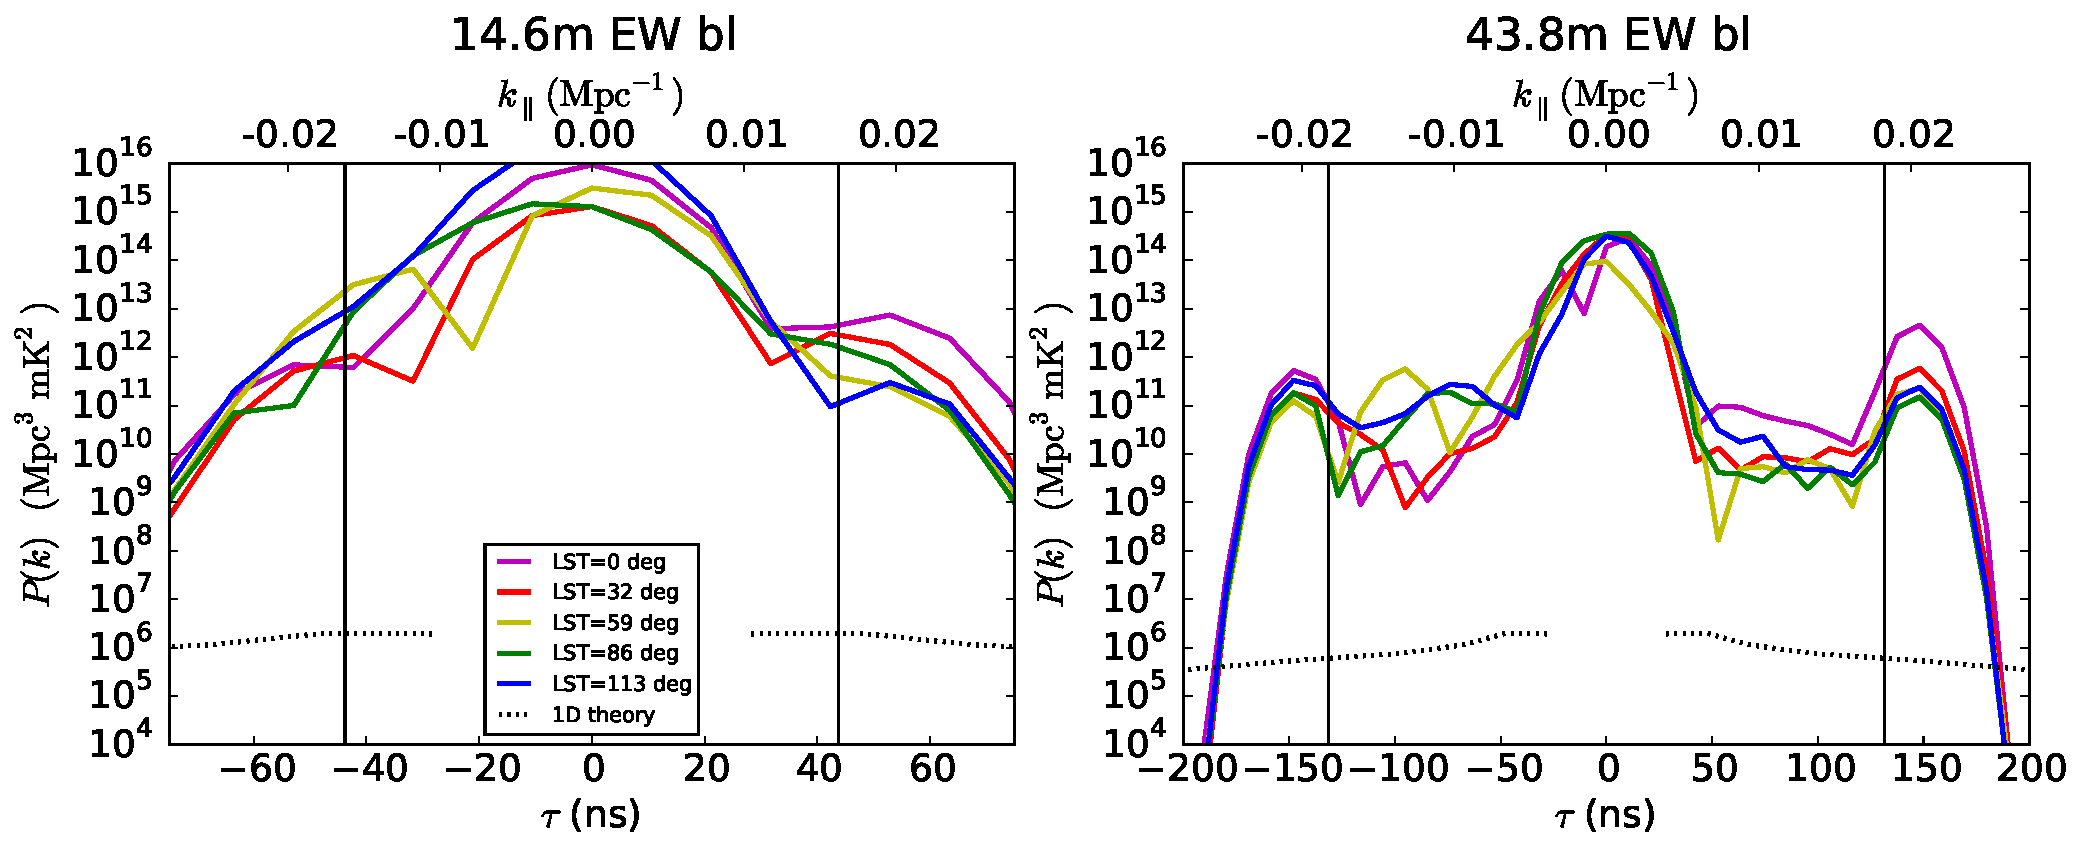
\includegraphics[width=6in]{nithya_fg_pspec_all_lst.pdf}
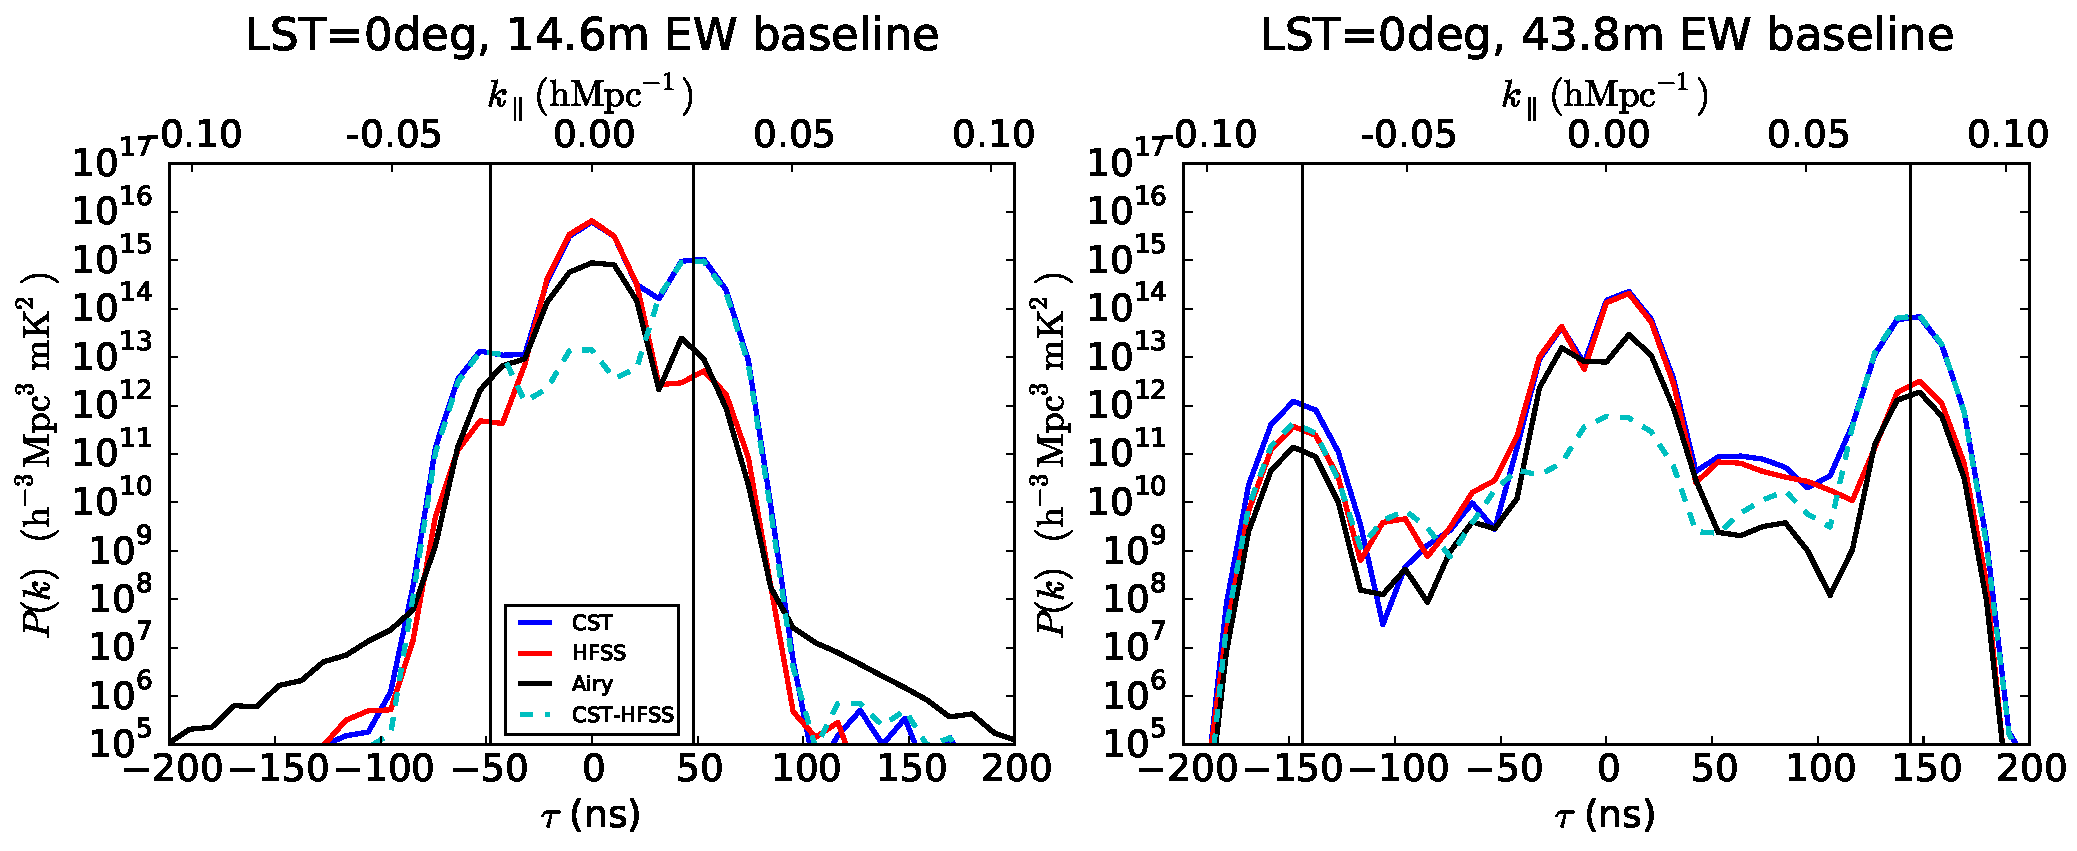
\includegraphics[width=6in]{nithya_fg_pspec_lst0deg.pdf}
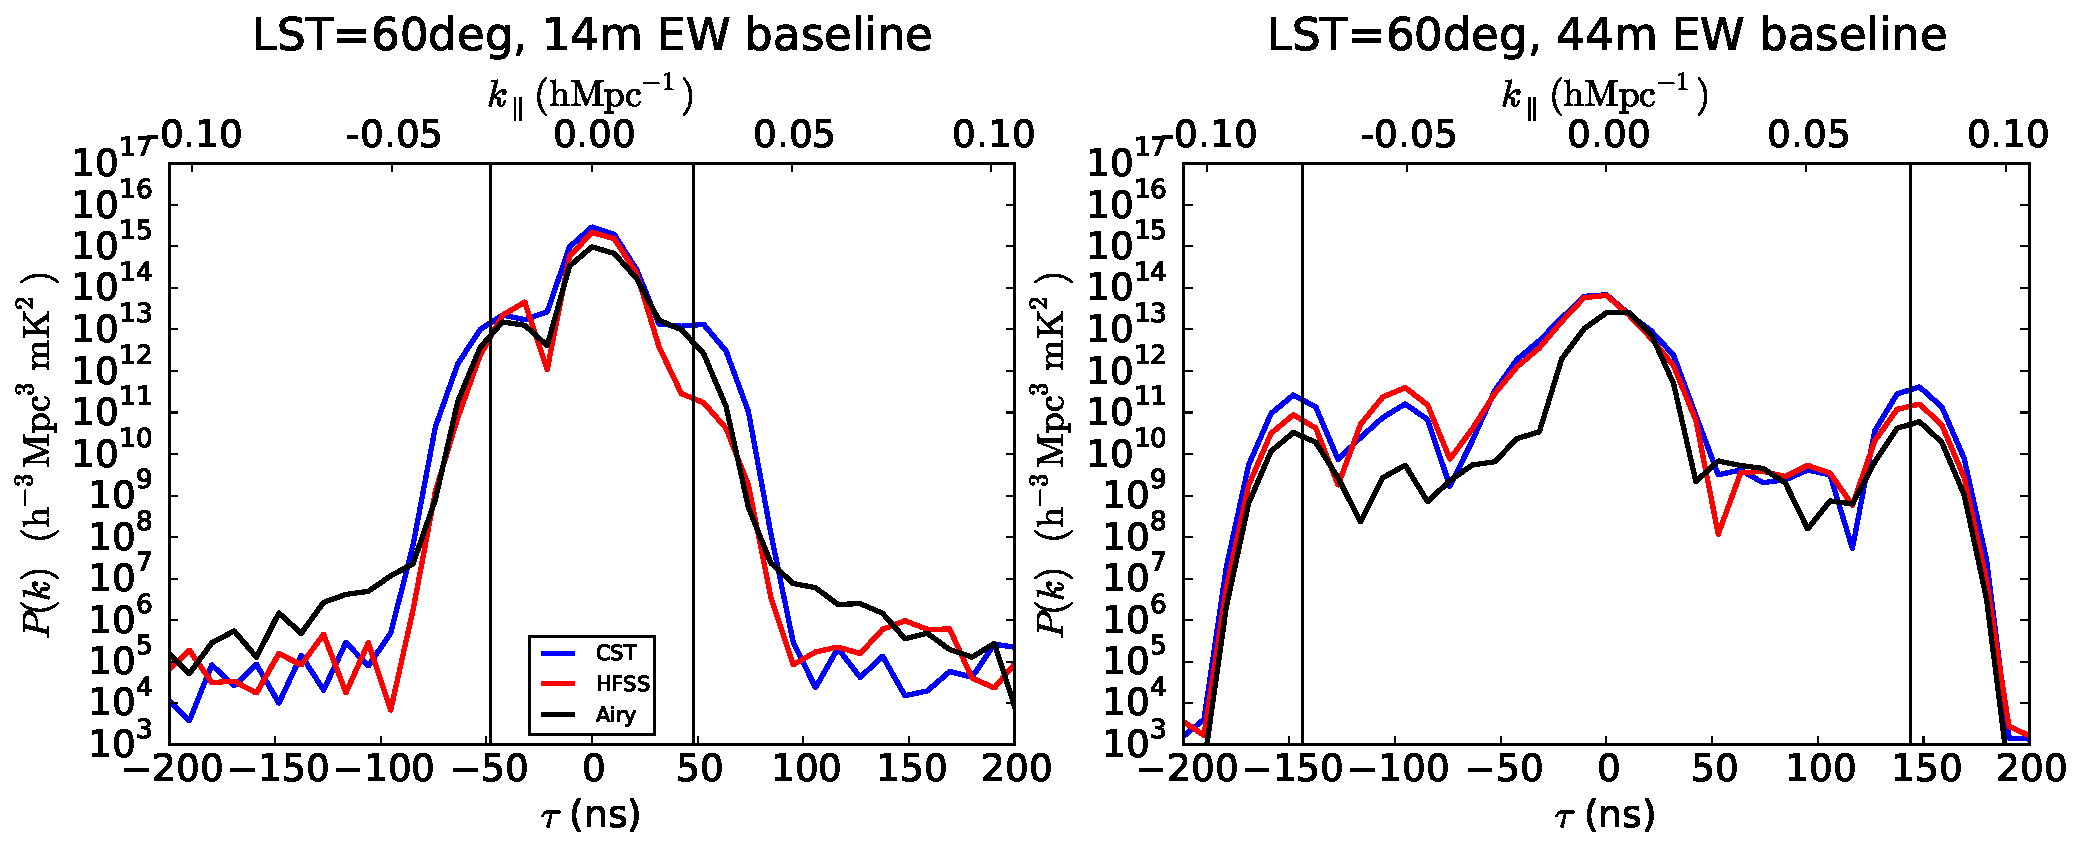
\includegraphics[width=6in]{nithya_fg_pspec_lst60deg.pdf}
\caption{Simulated foreground delay spectra using the HFSS beam at various LSTs (top panel). We also plot the delay spectra at two LSTs spanning the range of possible horizon brightening for three different beam models. The maximum horizon brightening at the positive horizon occurs close to 0$^\circ$ LST (middle panel), and the three beam models thus differ markedly in their predicted delay spectra near the horizon. In contrast, when the horizon brightening effect is smaller at 60$^\circ$ LST, the foreground delay spectra from all three beams agree much more closely.}
\label{fig:delayspec}
\end{figure*}

To characterize the effect of beam modeling uncertainties on this horizon brightening, we select two of these LSTs, one with maximal horizon brightening ($2^\circ$), and one with minimal horizon brightening ($62^\circ$). Figure \ref{fig:gsmplots} shows the sine-projected Global Sky Model, which dominates the horizon brightening effect, in horizontal coordinates with units of Kelvin for both LSTs. Dashed lines mark zenith angles 20$^\circ$, 40$^\circ$, 60$^\circ$, 80$^\circ$. These plots confirm that the large negative delay peak at the 0$^\circ$ LST is due to the center of the galaxy just above the horizon. In contrast several hours later, the galactic center is fully below the western horizon, leaving only a slight brightening near the eastern horizon due to the weaker galactic anticenter. 

\begin{figure*}[h]
\centering
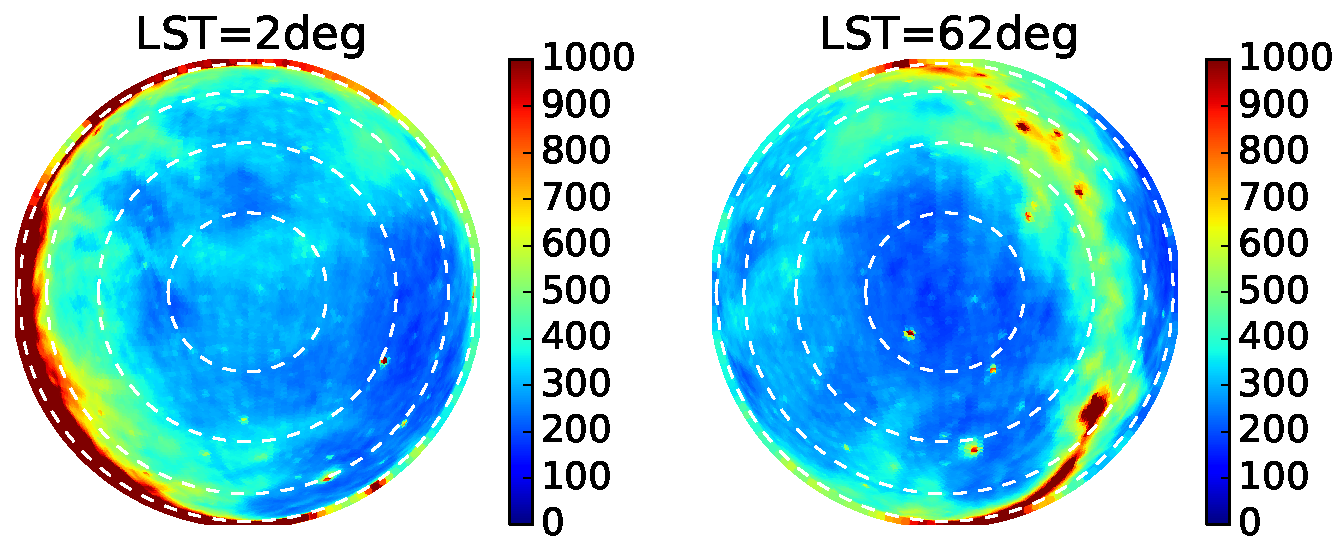
\includegraphics[width=6in]{gsm_kelvin_LST_2deg_and_62deg.pdf}
\caption{Global Sky Model \citep{gsm} in sine-projected horizontal coordinates at LST of 2$^\circ$ (left) and 62$^\circ$ right. The very bright emission from the center of the galaxy at the western horizon at 2$^\circ$ is seen in the delay spectra of EW baselines as a horizon brightening at negative delay.}
\label{fig:gsmplots}
\end{figure*}

How much do the predicted foreground power spectra differ between the three model dish power patterns? Figure \ref{fig:delayspec} (middle panel) shows the simulated delay spectra for all three beams at $0^\circ$ LST, when the horizon brightening is worst. Both numerical models agree out to delays of roughly 20\,ns on the 14.6\,m baseline and 50\,ns on the 43.8\,m baseline. These numbers suggest that the beams track each other fairly well out to 25$^\circ$ from zenith, beyond which they diverge. This is roughly what is observed in Figure \ref{fig:measuredbeamslices} (middle panel). At larger delays, especially near the positive delay horizon limit, all three model delay spectra diverge due to the significant edge brightening which effectively discriminates between these models. The CST, HFSS, and Airy beams reach roughly -35\,dB, -38\,dB, and -50\,dB at the horizon (Figure \ref{fig:modelbeams}), consistent with the fact that the CST beam has the largest horizon brightening, followed by the HFSS beam, and then by the Airy beam. This is seen in the delay spectra for both baseline lengths, though the edge brightening is much clearer on the longer baseline where it less diluted by zero delay emission.  

In contrast, all three model agree much more closely when there is little or no edge brightening as in Figure \ref{fig:measuredbeamslices} (bottom panel) where we plot the delay spectra for all three beams for 60$^\circ$ LST. There is still a modest flattening off near the horizon on the 14.6\,m baseline and a slight peak on the 43.8\,m baseline due to the large solid angle near the horizon. However as the near horizon emission at this LST is roughly the same temperature as emission from everywhere else on the sky, the difference between the three beam models is greatly reduced.

\section{Discussion}

%- power spectrum analyses by first generation instruments are ongoing, but face many challenges
%- that’s why HERA was designed to be optimized for 21cm

Power spectrum analyses by first generation 21\,cm observatories are ongoing, but are contending with challenges ranging from calibration and foreground modeling to the analysis effort required to process thousands of hours of data. HERA draws on the most successful ideas from these first generation instruments, pursuing a compact and redundant array layout and collecting area antenna elements to minimize analysis cost. The hexagonal grid allows redundant calibration and coherent power spectrum integration, and the large 14\,m dish achieves sufficient sensitivity at a reasonably data processing and analysis cost. The papers in this series characterize the 14\,m diameter dish used as HERA's antenna element using reflectometry measurements and simulations which probe its frequency response, as well as power pattern measurement which probe its angular response. 

%- in this paper we have characterized the HERA dish’s angular response
%  down to 60deg zenith angle, -35dB from zenith
%- confirms models to exquisite fidelity unachievable with celestial sources
%- the level of model disagreement also gives us a handle on antenna-to-to antenna variation

We present in this paper beam pattern measurements at 137\,MHz and discuss their implications for 21\,cm power spectrum analysis in terms of sensitivity and foreground isolation. We begin with the power pattern measurements using the beam mapping system of \citet{neben15} which we deploy at the prototype three-element HERA array at the National Radio Astronomy Observatory--Green Bank. Only one dish had been constructed when these measurements were made. We present measured power patterns for three dish configurations with the feed at different heights over the dish surface in order to characterize the focus of the system. The measured power patterns probe nearly two thirds of the visible sky, down to -30\,dB relative to the zenith response. The measured beams agree well with both models in the main lobe out to 10--20$^\circ$ from zenith, then roughly track the typical sidelobe levels at 20--30\,dB below zenith though fail to reproduce the exact sidelobe amplitudes and locations. 

These deviations away from models and away from 180$^\circ$ azimuthal symmetry are larger than the $\pm1$\,dB systematics observed in the null experiments which probe our beam measurement accuracy, suggesting they are genuine measurements of the in situ dish beam. The most likely dish non-idealities are dish surface imperfections and feed misalignment, both of which may vary from antenna to antenna in the full HERA array. Characterizing this antenna-to-antenna beam variation and its effects on power spectrum analyses for HERA, as Neben et al. (submitted) do for the MWA, is left as future work.

%% sensitivity
% collecting area 
% power spectrum SNR
We quantify HERA's 21\,cm power spectrum sensitivity given our beam measurements by first computing the collecting area of the different dish configurations. We observe a reduction of 30--50\% from the geometric cross section of a 14\,m dish due to the dipole feed and its cylindrical skirt which tapers the beam towards the edge of the dish to mitigate cross coupling with adjacent dishes. We convert these collecting areas into effective dish sizes, then use 21cmSense to predict the overall power spectrum SNR with one season of HERA-127 data. We find SNRs of 6--8 in pessimistic and moderate foreground scenarios, and 24--29 in optimistic ones, to be compared with SNRs of roughly 10 and 37 using full geometric collecting area. While certainly a reduction from the theoretical limit, these sensitivities still permit a very significant detection of the 21\,cm signal after a single observing season.

%% foreground delay spectrum simsulations
%- given the latest understanding of instrument chromaticity and
%  foreground isolation (ie, Nithya), we simulate the effects of these
%  beams on science
 %   - taking into account uncertainties in near-horizon beam response unprobed by our measurements
%- we make predictions for the level of horizon brightening at different LSTs, and discuss the uncertainties due to uncertain beam models (horizon brighting is an exquisite of the low elevation beam response, though an integrated statistic)
% horizon brightening will dominated leakage into the outer window modes
Beyond simple sensitivity considerations, though, the beam pattern affects science analyses by reweighting celestial emission in different regions of the sky, which are then imprinted with different frequency dependence by the interferometer. Longer baselines are proportionately more susceptible to this effect, giving rise to a ``wedge'' shaped region in 2D Fourier space. \citet{nithya15} has highlighted that the distribution of foregrounds \textit{within} the wedge is important as well. If the beam response is sufficiently shallow at low elevations, there is a brightening of emission from near the horizon in line with the baseline due in part to the large solid angle at low elevations. This produces a characteristic ``pitchfork'' shape in the delay spectrum of a single baseline, with a zero delay peak due to bright near-zenith emission surrounded by tines at the negative and positive horizon limits due to emission from the two horizon directions in line with the baseline. These horizon peaks are \textit{most} at risk of leaking foreground power into the EOR window given chromatic instrumental imperfections such as bandpass miscalibration. 

We predict the magnitude of this effect for the HERA element as well as its dependence on beam modeling uncertainties. As expected, we find that the level of horizon brightening is largest when the galaxy is just above the horizon, and lowest when it is well below. When the pitchfork effect is large, its uncertainty is also large as seen in the deviation of the delay spectra with HFSS and CST beam models in these simulations. When the effect is small, the two beam models produce much more similar results, highlighting the delay spectrum as an exquisite probe of the challenging to measure beam response at very low elevations.

% frequency dependence of the beam pattern and overall gain (due to reflections) likely dominates leakage deep within the window, but the other papers in this series demonstrate that this leakage level is within our spec

As discussed by the other papers in this series, the frequency dependence of the beam power pattern and its overall gain widen the delay kernel of a source, leaking power into the EOR window. These papers demonstrate that in the best case, a combination of bandpass calibration and delay space CLEANing can mitigate foregrounds to a manageable level, while in the worst case, HERA can still achieve a XX--XX $\sigma$ detection of the EOR parameters from the power spectrum by simply excluding a very conservative buffer outside the wedge. All these considerations highlight the need for precision characterization of antenna elements and their implications for 21\,cm science analyses on the part of next generation observatories if we are to have any hope of making this challenging measurement.





%% The reference list follows the main body and any appendices.
%% Use LaTeX's thebibliography environment to mark up your reference list.
%% Note \begin{thebibliography} is followed by an empty set of
%% curly braces.  If you forget this, LaTeX will generate the error
%% "Perhaps a missing \item?".
%%
%% thebibliography produces citations in the text using \bibitem-\cite
%% cross-referencing. Each reference is preceded by a
%% \bibitem command that defines in curly braces the KEY that corresponds
%% to the KEY in the \cite commands (see the first section above).
%% Make sure that you provide a unique KEY for every \bibitem or else the
%% paper will not LaTeX. The square brackets should contain
%% the citation text that LaTeX will insert in
%% place of the \cite commands.

%% We have used macros to produce journal name abbreviations.
%% AASTeX provides a number of these for the more frequently-cited journals.
%% See the Author Guide for a list of them.

%% Note that the style of the \bibitem labels (in []) is slightly
%% different from previous examples.  The natbib system solves a host
%% of citation expression problems, but it is necessary to clearly
%% delimit the year from the author name used in the citation.
%% See the natbib documentation for more details and options.

\bibliography{DishBeamMeasurements}


\end{document}
